\documentclass[pdf]{beamer}

%Subhi's styles
%\usecolortheme{whale}
%\usecolortheme{orchid}
%\useinnertheme[shadow]{rounded}
%\useoutertheme{infolines}

%%Alternative
%\usetheme{Warsaw}

\usetheme{Madrid}

\usepackage{pgfpages}
%\setbeameroption{show notes on second screen}
%\setbeameroption{show notes}


\DeclareMathOperator{\Tr}{Tr}
\DeclareMathOperator{\prox}{prox}
\newcommand{\avg}[1]{\mbox{$\left\langle \, #1 \, \right\rangle$}}
\newcommand{\qav}[1]{\mbox{$\left\langle\left\langle \, #1 \, \right\rangle\right\rangle$}}
\newcommand{\ra}{\rightarrow}





%\mode<presentation>{}


\title[Physics of Learning]{4th year Review - Statistical Physics Perspectives on Learning in High Dimensions}
\subtitle{Advisor: Surya Ganguli}

\author{Madhu Advani}
\institute{Stanford University}

\begin{document}

\begin{frame}
    \titlepage
\end{frame}

%---------------------Frame----------------
\begin{frame}{Outline}
\begin{block}{Current Research}
Optimal Tractable High Dimensional M-estimation
\end{block}
\vspace{.1in}
\begin{block}{Future Directions}
    \begin{enumerate}
        \item LN and GLM extensions of M-estimation also Optimal Signal Processing (Structured Coefficients)
        \item Random Dimensionality Reduction
        \item Phase transitions in clustering Behavior
    \end{enumerate}
\end{block}
\vspace{.1in}
\begin{block}{Previous Research and Future Plan}
    \begin{enumerate}
        \item Review Paper
        \item Timeline
    \end{enumerate}
\end{block}
\end{frame}


%------------Frame------------
\begin{frame}{Problem Setup}
\begin{itemize}
\item Consider Statistical inference with $N$ data points and $P$ unknowns (predictors).
\item (Easy) Classical Regime: $\kappa = P/N\ra 0$
\item (Hard) High Dimensional Regime: $\kappa = P/N \ne 0$

\end{itemize}
\vspace{.2in}


Outputs generated by:
$y_i = \mathbf{X_i}\cdot \mathbf{w^0} + \epsilon_i \quad \quad i\in [1,\dots N]$

\vspace{.2in}
\begin{itemize}
\item We want to find $\mathbf{w^0}\in \mathcal{R}^P$
\item Noise $\epsilon$ not necessarily gaussian

\end{itemize}


\begin{equation*}
\mathbf{\hat{w}}=\arg \min_{\mathbf{w}}{\left[ \sum_{i} {\rho\left( y_i - \mathbf{X}_{i} \cdot \mathbf{w}\right)}\right]}
\end{equation*}

E.g. $\rho(x) = x^2,|x|,-\ln f(x)$

\end{frame}
%-----------------------------


%----------------Frame-------------------
\begin{frame}{Maximum Likelihood}




\end{frame}
%----------------------------------










%-----------------Frame-------------
\begin{frame}[t]{Classical vs High Dimensional Optimal M-estimation}

    \begin{block}{Classical}
        \begin{itemize}
        \item $N\ra \infty$, $P/N =\kappa \ra 0$
        \vspace{.1in}
        \item $\rho_{\text{opt}} = -\log f$
        \vspace{.1in}
        \item $\qav{(\hat{w}_i-w^0_i)^2} \ge \frac{\kappa}{\int{\frac{f'^2}{f}}}$
        \vspace{.1in}
        \end{itemize}

    %\begin{flushright} $\epsilon_a \sim f$ \end{flushright}
    \end{block}


    \begin{block}{High Dimensional}
        \begin{itemize}
        \item $N,P\ra \infty$, $P/N =\kappa \in [0,1]$
        \vspace{.1in}
        \item $\rho_{\text{opt}}(x) = -\inf_y{\left[\ln(\zeta_{\hat{q}_0}(y))+\frac{(x-y)^2}{2 \hat{q}_0}\right]} \quad \quad \quad \quad \zeta = f*\phi_{\hat{q}_0}$
        \vspace{.1in}
        \item $\qav{(\hat{w}_i-w^0_i)^2} \ge \frac{\kappa}{\int{\frac{\zeta'^2}{\zeta}}}$
        \vspace{.1in}
        \end{itemize}
    \end{block}
\end{frame}
%------------------------------------








%------------------------------------------------

%%---------------------Frame----------------
%\begin{frame}{Background}
%
%\begin{block}{Motivation}
%\begin{itemize}
%\vspace{.2in}
%\item{Consider Estimating $N$ parameters with $T$ samples}
%\vspace{.2in}
%\item{Maximum Likelihood is guaranteed to be optimal for finite $N$ as $T\rightarrow \infty$: $ \frac{N}{T}\ra 0$}
%\vspace{.2in}
%\item{A better approximation is the high dimensional limit: $N,T\ra \infty$ with $\frac{N}{T}\ra \kappa$} (Data Deluge)
%\vspace{.2in}
%\item{What is the best Inference Algorithm in this regime?}
%
%\end{itemize}
%\end{block}
%\end{frame}
%%------------------------------------------------




%%-----------Slide-----------------------------------
%\begin{frame}[t]{M-estimation Problem Statement}
%
%    \begin{block}{Inference Formulation}
%
%    \parbox{.40\textwidth}{
%        Consider $y_i$ drawn from
%        \begin{equation*}
%        y_i = \mathbf{X_i} \cdot \mathbf{w^0} + \epsilon_i
%        \end{equation*}
%
%
%    }
%    \parbox{.55\textwidth}{
%
%        \begin{flushright}
%        Known: $\mathbf{y}\in \mathcal{R}^N, \mathbf{X}\in \mathcal{R}^{N \times P}$ \\
%        \vspace{.1in}
%        Unknown: $\boldsymbol{\epsilon} \in \mathcal{R}^N$, $\mathbf{w^0}\in \mathcal{R}^P$
%        \\
%               \vspace{.1in}
%        iid Known Distribution: $\epsilon_i \sim f, w^0_j \sim g$,
%
%        $X_{ij}\sim \mathcal{N}(0,\frac{1}{P})$
%        \end{flushright}
%    }
%    %\begin{flushright} $\epsilon_a \sim f$ \end{flushright}
%    \end{block}
%
%
%    \begin{columns}
%
%    \begin{column}{.35\textwidth}
%        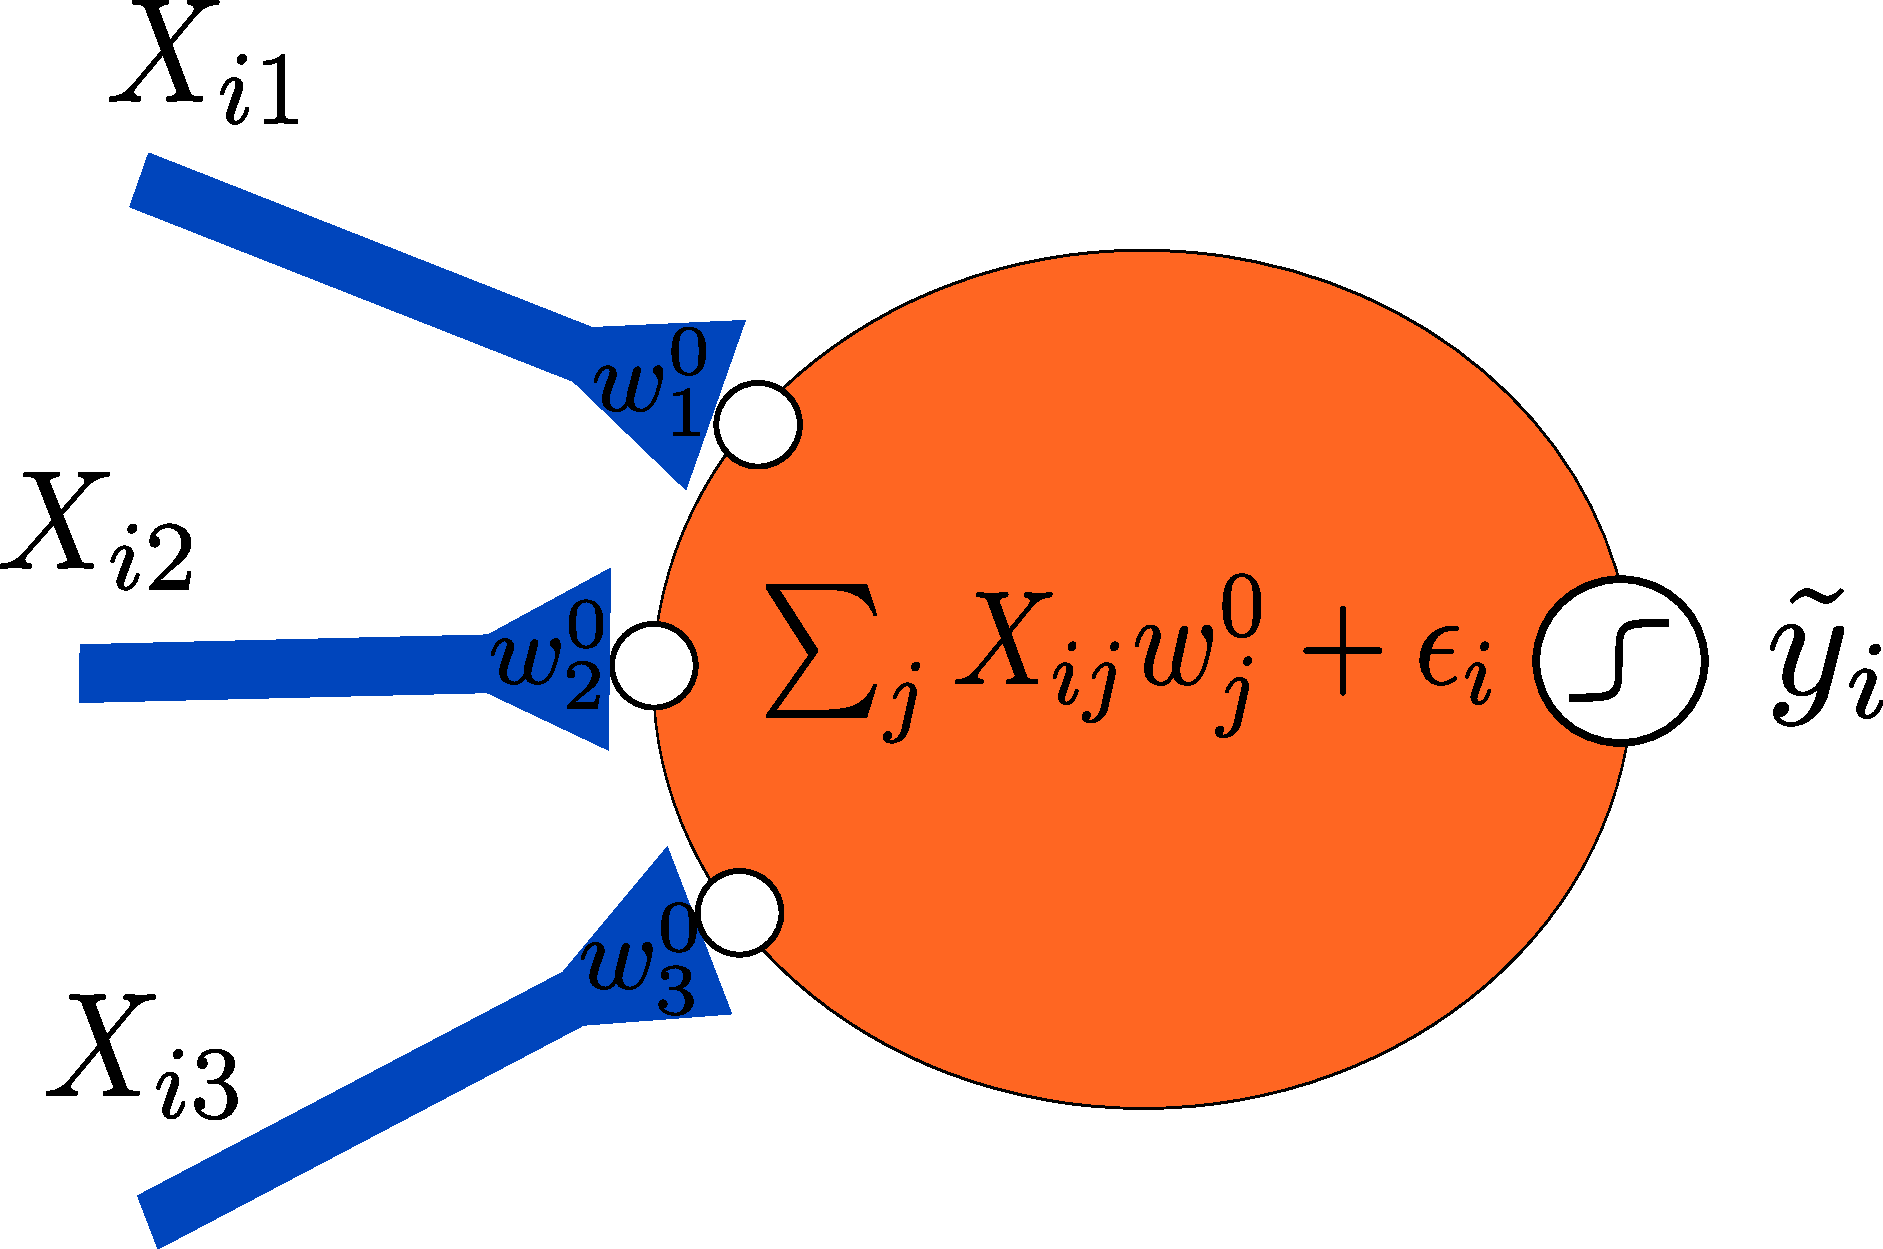
\includegraphics[width = .7\linewidth]{neuronInference.pdf}
%
%
%    \end{column}
%
%    \begin{column}{.60\textwidth}
%    \begin{block}{M-estimation}
%    \begin{equation*}
%        \mathbf{\hat{w}}=\arg \min_{\mathbf{w}}{\left[ \sum_{i} {\rho\left( y_i - \mathbf{X}_{i} \cdot \mathbf{w}\right)}\right]}
%    \end{equation*}
%
%
%
%    \end{block}
%    E.g. $\rho(x) = x^2,|x|,-\ln f(x)$
%    \end{column}
%
%
%
%    \end{columns}
%\end{frame}
%%------------------------------------
%
%
%
%
%
%
%
%
%
%
%
%
%
%%-----------Slide-----------------------------------
%\begin{frame}[t]{Low Dimensional Optimal M-estimation}
%    \note{First I'll describe what happen the classical (low-dimensional theory)}
%    \begin{block}{Classical}
%       \begin{itemize}
%        \item $N\ra \infty$, $P/N =\kappa \ra 0$
%        \vspace{.1in}
%        \item $\rho_{\text{opt}} = -\ln f$
%        \vspace{.1in}
%        \item $\qav{(\hat{w}_i-w^0_i)^2} \ge \frac{\kappa}{\int{\frac{f'^2}{f}}}$
%        \vspace{.1in}
%        \end{itemize}
%
%
%    \end{block}
%    \vspace{.3in}
%
%    \begin{columns}
%
%    \begin{column}{.35\textwidth}
%        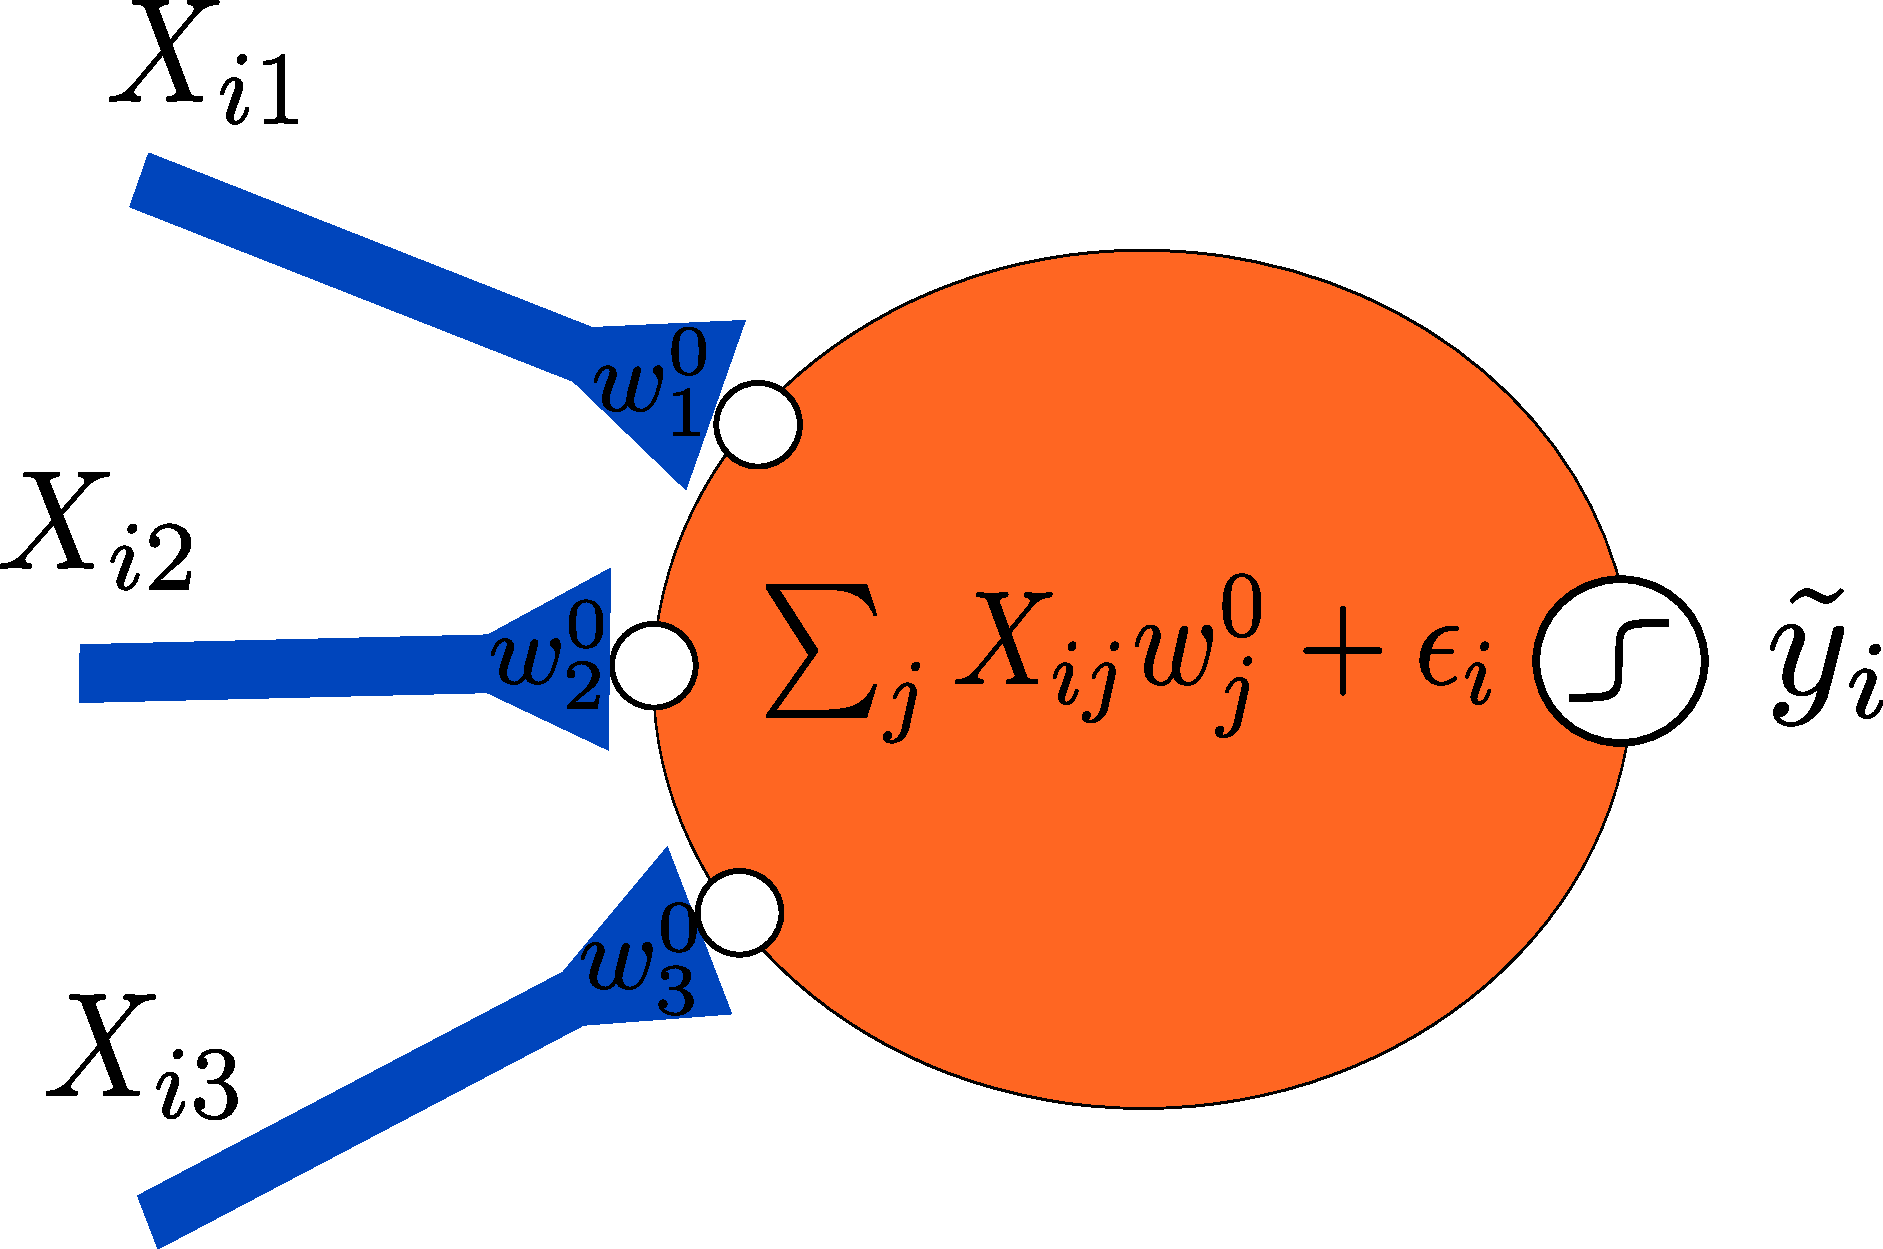
\includegraphics[width = .7\linewidth]{neuronInference.pdf}
%
%
%    \end{column}
%
%    \begin{column}{.60\textwidth}
%        The optimal policy approaches Maximum Likelihood, satisfying Cramer-Rao bound.
%    \end{column}
%
%
%
%    \end{columns}
%
%
%\end{frame}
%%------------------------------------
%
%\begin{frame}[t]{M-estimation in the Data Deluge Regime}
%
%    \begin{block}{High Dimensional}
%        \begin{itemize}
%        \item $N,P\ra \infty$, $P/N =\kappa \in [0,1]$
%        \vspace{.1in}
%        \item $\rho_{\text{opt}}(x) = -\inf_y{\left[\ln(\zeta(y))+\frac{(x-y)^2}{2 \hat{q}_0}\right]} \quad \quad \quad \quad \zeta = f*\phi_{\hat{q}_0}$
%        \vspace{.1in}
%        \item $\qav{(\hat{w}_i-w^0_i)^2} \ge \frac{\kappa}{\int{\frac{\zeta'^2}{\zeta}}}$
%        \vspace{.1in}
%        \end{itemize}
%    \end{block}
%
%    \vspace{.3in}
%    \begin{columns}
%
%    \begin{column}{.35\textwidth}
%        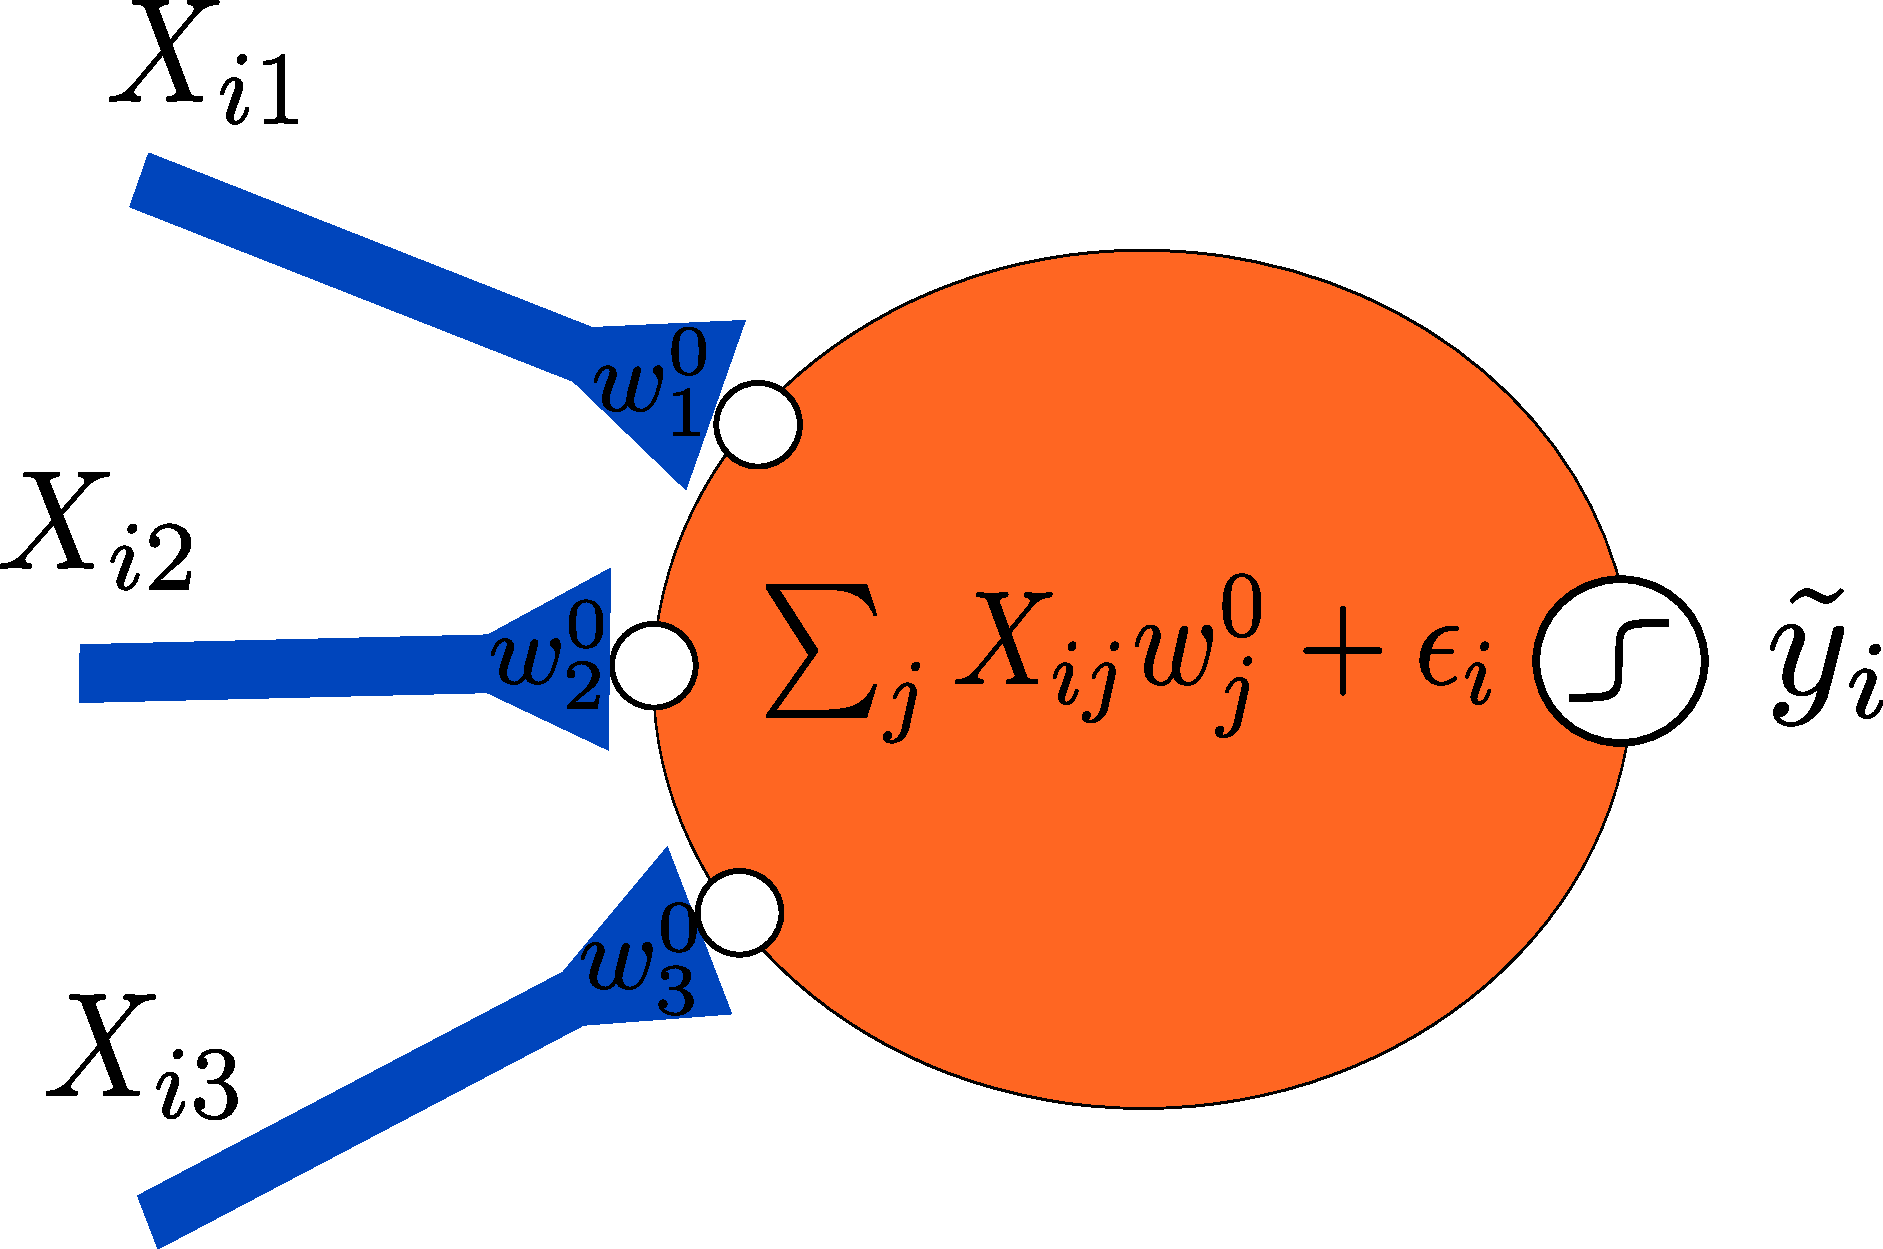
\includegraphics[width = .7\linewidth]{neuronInference.pdf}
%    \end{column}
%
%    \begin{column}{.60\textwidth}
%        The optimal policy is no longer Maximum Likelihood! A stronger inequality than Cramer-Rao bound holds.
%    \end{column}
%
%    \end{columns}
%\end{frame}
%
%
%\begin{frame}{Classical vs High Dimensional}
%
%\begin{itemize}
%       \vspace{.1in}
%     \item{Maximum Likelihood is the optimal M-estimator for $P/N\ra 0$}
%     \vspace{.1in}
%     \item{El Karoui, et. al. recently demonstrated new phenomena for $P/N \ra \kappa$ as $P,N \ra \infty$: Modified Loss Function and Confidence Intervals in the Big Data Limit}
%\end{itemize}
%
%
%\end{frame}
%
%
%
%








%-----------Slide-----------------------------------
\begin{frame}[t]{Adding a Regularizer}
    \note{Maximum Likelihood is based on finding the mode of data given the coefficients. Especially in the high dimensional regime, where a prior can really help us, we want to find the mode of the coefficients given the data!}

    \begin{equation*}
        P(\mathbf{w^0}|\mathbf{X},\mathbf{y}) = \frac{P(\mathbf{X},\mathbf{y}|\mathbf{w^0})P(\mathbf{w^0})}{P(\mathbf{X},\mathbf{y})}
    \end{equation*}

    \begin{block}{Maximum a Priori}
        \begin{equation*}
            \small{\mathbf{\hat{w}_{\text{MAP}}} =\arg\min_{\mathbf{w}}{\left[\sum_i{-\log f(y_i - \mathbf{X}_i\cdot \mathbf{w})} +\sum_j{-\log{g(w_j)}}\right]}}
        \end{equation*}
    \end{block}

    \begin{block}{Regularized M-estimation}
    \begin{equation*}
        \mathbf{\hat{w}}=\arg \min_{\mathbf{w}}{\left[ \sum_{i} {\rho\left( y_i - \mathbf{X}_{i} \cdot \mathbf{w}\right)} + \sum_j{\sigma(w_j)}\right]}
    \end{equation*}
    Note separability. Solvable for convex strategy $\sigma,\rho$
    \end{block}

\end{frame}
%------------------------------------



%-------------Frame--------------------
\begin{frame}{Motivation}

\begin{equation*}
            \mathbf{\hat{w}} = \arg\min_\mathbf{w} {\sum_a{\rho(y_a - \mathbf{X_a} \cdot\mathbf{ w})} + \sum_i{\sigma(w_i)}}
        \end{equation*}

\begin{block}{Applications}
\begin{itemize}
 \item{Maximum Likelihood (ML) and MAP commonly applied to High Dimensional Bio-informatics problems, where we should expect poor performance}
 \item{Deriving/Understanding the Optimal M-estimator has potential applications for statistical inference and signal processing.}
 \item{ Tractability of this form of optimization popular: Compressed Sensing, LASSO, Elastic Net}
\end{itemize}
\end{block}


%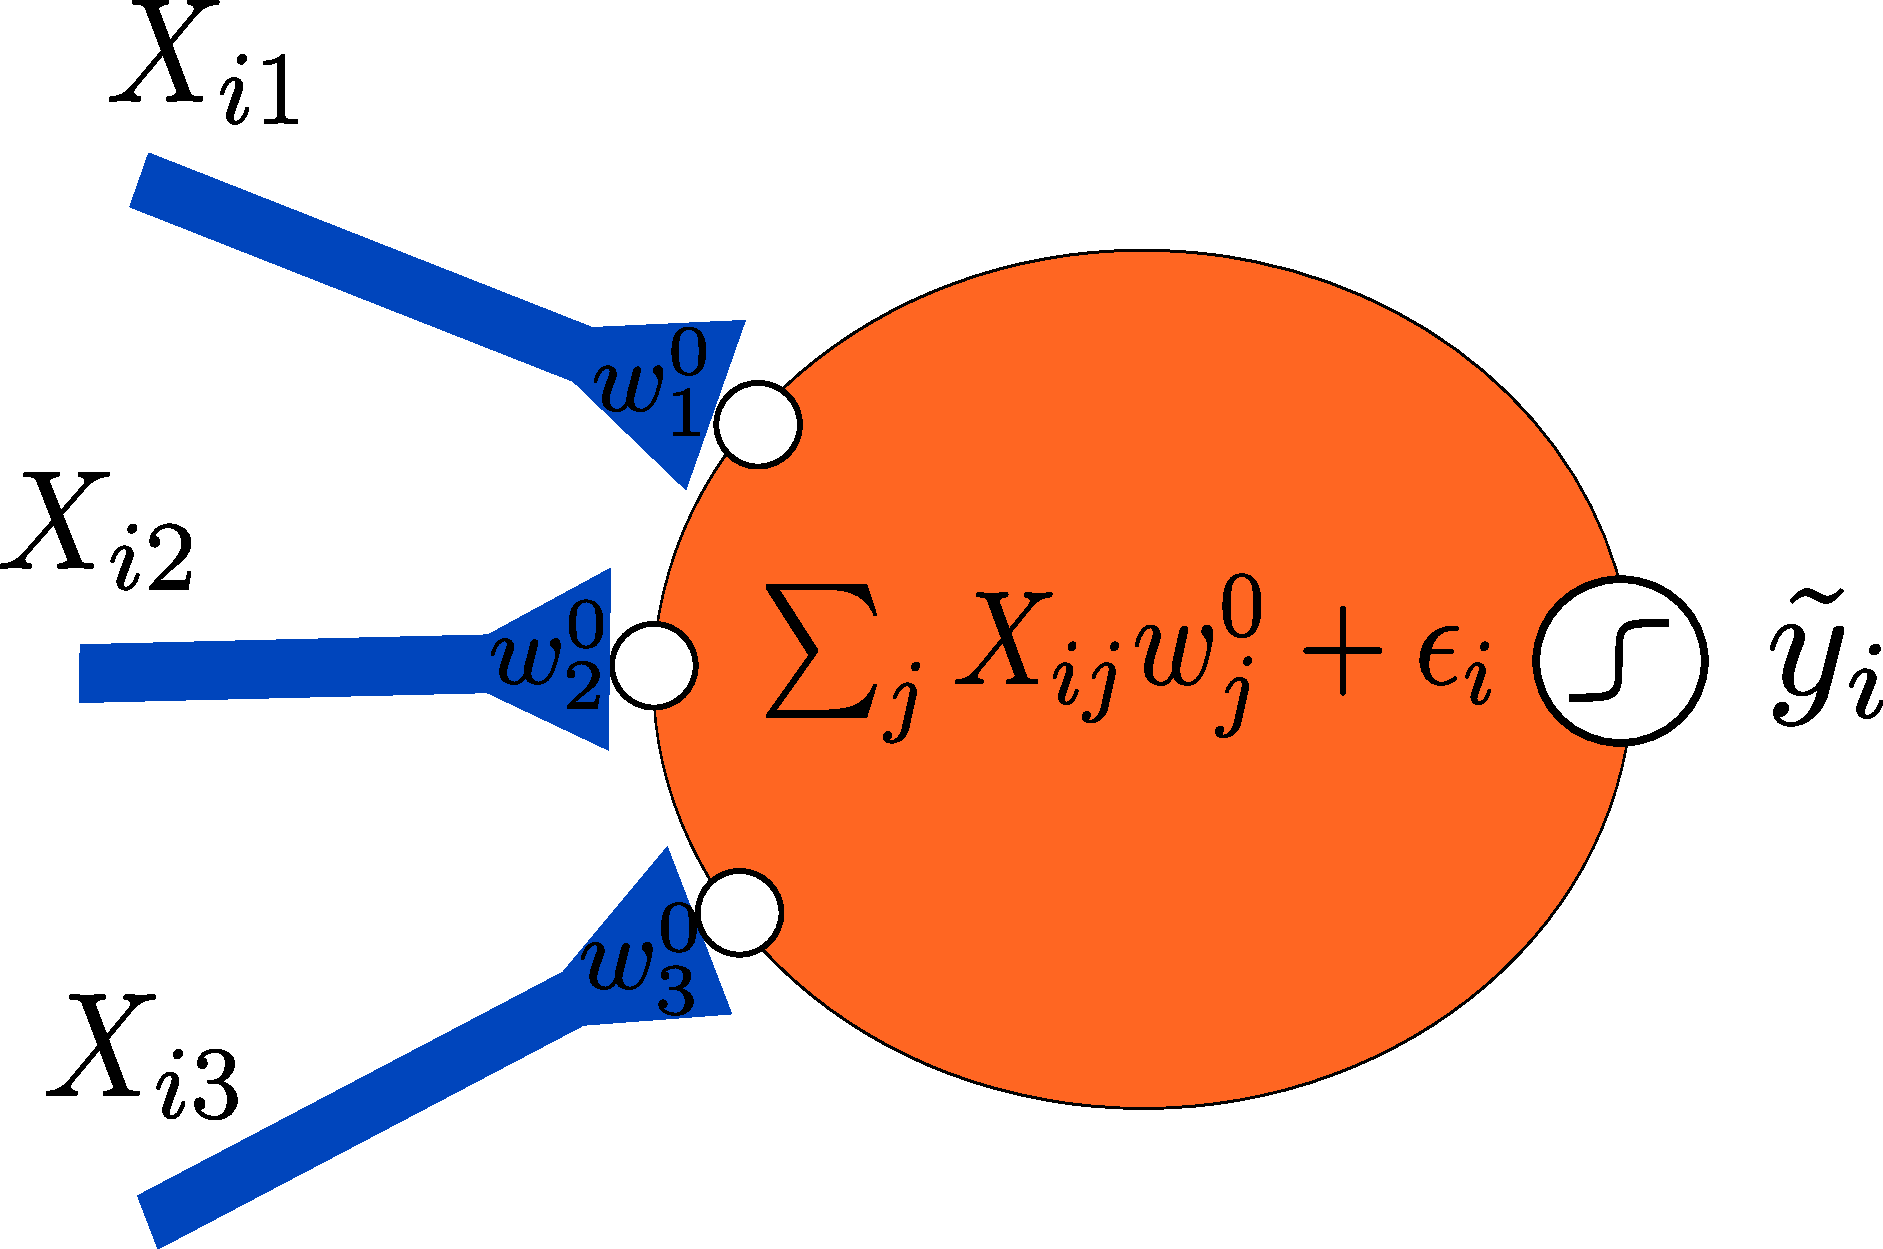
\includegraphics[width = .4\linewidth]{neuronInference.pdf}



\end{frame}
%----------------------------------------



%%-----------Slide-----------------------------------
%\begin{frame}[t]{Background and Motivation}
%    \begin{block}{Background}
%        \begin{itemize}
%            \item{Maximum Likelihood is the optimal M-estimator for $P/N\ra 0$}
%            \item{El Karoui, et. al. recently demonstrated new phenomena for $P/N \ra \kappa$ as $P,N \ra \infty$: Modified Loss Function and Confidence Intervals in the Big Data Limit}
%        \end{itemize}
%    \end{block}
%
%    \begin{block}{Motivation}
%        \begin{itemize}
%            \item{Formulate and solve this optimization problem in a Statistical Physics framework}
%            \item{Maximum Likelihood and MAP are applied to High Dimensional Bio-informatics problems where they may give poor performance- can we quantify and optimize this?}
%            \item{ Deriving the Optimal regularized M-estimator: potential applications for big data inference and signal processing.}
%        \end{itemize}
%
%    \end{block}
%
%    \begin{equation*}
%        P(\mathbf{w^0}|\mathbf{X},\mathbf{y}) = \frac{P(\mathbf{X},\mathbf{y}|\mathbf{w^0})P(\mathbf{w^0})}{P(\mathbf{X},\mathbf{y})}
%    \end{equation*}
%
%    \begin{block}{Maximum a Priori}
%        \begin{equation*}
%            \small{\mathbf{\hat{w}_{\text{MAP}}} =\arg\min_{\mathbf{w}}{\left[\sum_i{-\log f(y_i - \mathbf{X}_i\cdot \mathbf{w})} +\sum_j{-\log{g(w_j)}}\right]}}
%        \end{equation*}
%    \end{block}
%
%\end{frame}
%%------------------------------------

%%--------------------Slide-----------
%\begin{frame}[t]{Inference Algorithm}
%
%    Beyond Maximum Likelihood and MAP
%    \vspace{.2in}
%
%    \begin{block}{M-estimation for Inference}
%        \begin{equation*}
%            \mathbf{\hat{w}} = \arg\min_\mathbf{w} {\sum_a{\rho(y_a - \mathbf{X_a} \cdot\mathbf{ w})} + \sum_i{\sigma(w_i)}}
%        \end{equation*}
%    \end{block}
%
%    \vspace{.2in}
%    Note that:
%
%    \begin{itemize}
%
%        \item{This form allows us to encompasses MAP and ML}
%        \vspace{.1in}
%        \item {Assuming convex loss and regularization functions, this problem is tractable and solutions are unique}
%        \vspace{.1in}
%        \item{Examples include Compressed Sensing, Lasso, Elastic Net}
%    \end{itemize}
%\end{frame}
%%------------------------------------




%------------------------Frame------------
\begin{frame}[t]{Statistical Physics Formulation}
Define a spin glass system to solve M-estimator inference

\begin{block}{Spin Glass System}
Define continuous spins $\mathbf{u}=\mathbf{w^0}-\mathbf{w}$. Let the Energy of the system be a function of these spins

\begin{equation*}
 E_{\boldsymbol{\Lambda}}(\mathbf{u})=\sum_i{\rho\left(\mathbf{X}_{i}\cdot \mathbf{u} +\epsilon_i\right)}+\sum_a{\sigma(w^0_a-u_a)}
\end{equation*}

%with Gibbs distribution


This in turn induces an equilibrium probability distribution on the state

\begin{align*}
P_{G}(\mathbf{u}) &= \frac{e^{-\beta E_{\boldsymbol{\Lambda}}(\mathbf{u})}}{Z_{\boldsymbol{\Lambda}}} & Z_{\boldsymbol{\Lambda}} &= \int{e^{-\beta E_{\boldsymbol{\Lambda}} (\mathbf{u}) }du}
\end{align*}


%The solution of our M-estimator problem occurs in the low temperature limit, and convexity guarantees

\begin{equation*}
\lim_{\beta \rightarrow \infty} P_{G}(\mathbf{u}) = \delta\left(\mathbf{u} - \mathbf{w^0} +\mathbf{\hat{w}}\right)
\end{equation*}

\end{block}


\end{frame}
%------------------------------------







%---------------------
\begin{frame}{Replica Solution}


\begin{block}{\begin{center}Coupled Equations Relating Order Parameters\end{center}}
\begin{equation*}
\qav{\left(\prox_{c\rho}{(\sqrt{q} z + \epsilon)} -\sqrt{q}z -\epsilon\right)^2}_{z,\epsilon}= \kappa q
\end{equation*}


\begin{equation*}
\qav{\prox_{c\rho}'(\sqrt{q}z + \epsilon)}_{z, \epsilon} = 1-\kappa
\end{equation*}
\end{block}




\parbox{.40\textwidth}{
\begin{block}{Order Parameters}
$q =$
$c =$
\end{block}
}\parbox{.38\textwidth}{
\begin{center}	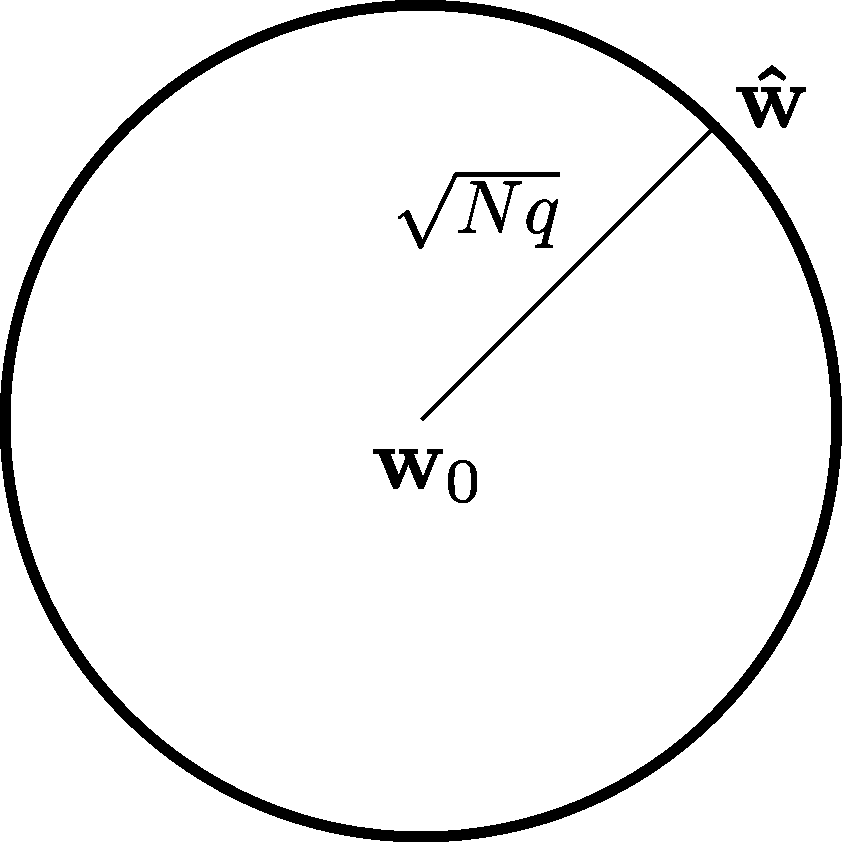
\includegraphics[width=0.5in]{errorCircle.pdf}
\end{center}
}

%\parbox{.45\textwidth}{
%\begin{center} 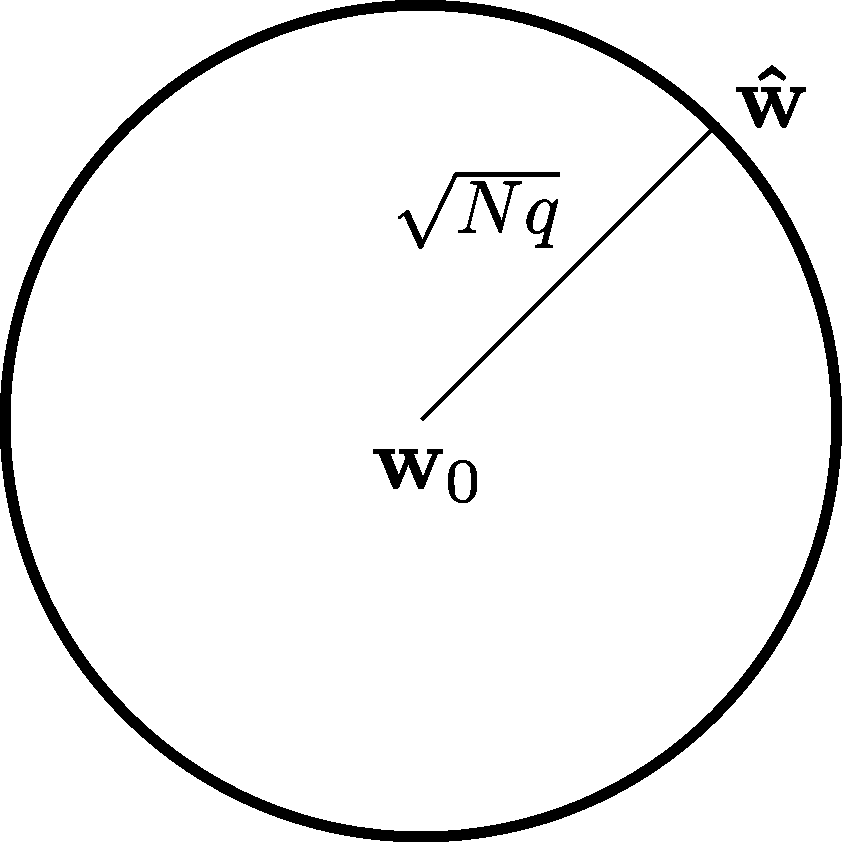
\includegraphics[width=0.4\linewidth]{errorCircle.pdf}
%\end{center}
%}



\end{frame}


%------------------------------

\begin{frame}{Proximal Map}


\begin{block}{Definition}
\begin{equation*}
prox_f(x) = \arg\min_y \left[\frac{(x-y)^2}{2} + f(y)\right]
\end{equation*}

\begin{equation*}
= \left[I + \partial f\right]^{-1} (x)
\end{equation*}


\end{block}
\vspace{.2 in}

\begin{itemize}
\item{Note that both $f$ and $\prox_f$ are functions}
\vspace{.2 in}

\item{Known for many functions: e.g. soft thresholding operator for L1 norm}

\vspace{.2 in}

\item{Used in proximal algorithms: minima of $f  \Leftrightarrow$ fixed points $ prox_f$}

\end{itemize}

\end{frame}
%----------------------------------------

%-------------Slide---------------
\begin{frame}{}
\begin{minipage}{.45\textwidth}

    \begin{block}{Order Parameters}
        nothing here yet
    \end{block}

\end{minipage}
\begin{minipage}{.45\textwidth}

    \begin{center}
        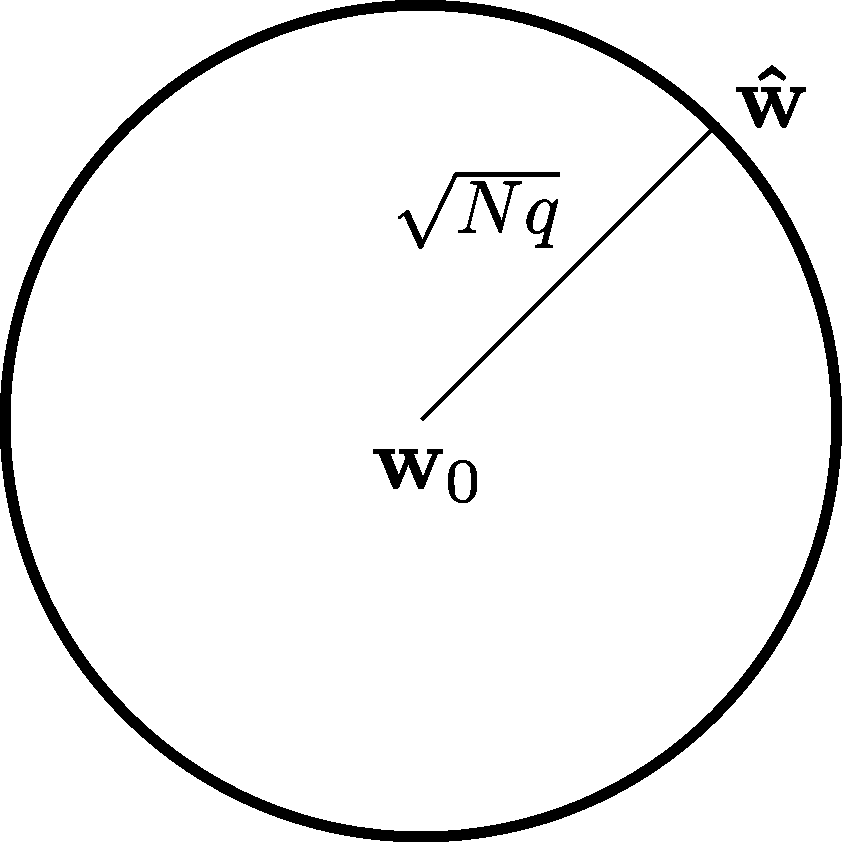
\includegraphics[width =.9in]{errorCircle.pdf}
    \end{center}

\end{minipage}




\end{frame}
%----------------------------------------





%-----------Slide-----------------------------------
\begin{frame}[t]{Unregularized M-estimators}

    \begin{itemize}
    \item $X_{ij}\in \mathcal{N}(0,1/P)$
    \item $\rho$ convex 
    \item $\epsilon$ iid
    \end{itemize}

    \vspace{.2in}
    
    \begin{block}{Optimal M-estimator}
        \begin{align*}
            \rho_{\text{opt}}(x) &= -\inf_y{\left[\ln(\zeta_{\hat{q}}(y))+\frac{(x-y)^2}{2 \hat{q}}\right]} & \zeta_{\hat{q}} &= f*\phi_{\hat{q}}
        \end{align*}
        \begin{align*}
           \hat{q} = \min{q} \quad \quad \text{s.t.} \quad q I_{q} &=\kappa & I_{q} = \int_{-\infty}^{\infty}{\frac{\zeta_{q}'^2(y)}{\zeta_{q}(y)}dy}
        \end{align*}


        \begin{itemize}
        \vspace{.1in}
        \item Best possible asymptotic Mean squared error for any convex M-estimator is $\hat{q}$
            \vspace{.1in}
        \item log-concave noise $f$ assumption
        \end{itemize}

    \end{block}

\end{frame}
%------------------------------------










\end{document} 